% questions.tex —— 2015 年·陕西卷·理工农医类 · 题目内容片段（无答案）
% 由 tools/generate_projects.py 依来源总账自 2015/2015_数学真题_陕西理_试题.md 生成，勿手改（改源 MD 后重跑）


\begin{gktip}
固定副本两页，未见答案、分值或选做说明；来源身份待核。第19题往返联合分布未明，答案待核。
\end{gktip}

\gkpart{一、选择题}

\begin{question}
\gkti{1}

设集合 $M=\{x\mid x^2=x\}$，$N=\{x\mid\lg x\leq0\}$，则 $M\cup N=$（　）。

   （A）$[0,1]$　（B）$(0,1]$　（C）$[0,1)$　（D）$(-\infty,1]$

\Needspace{0.4\textheight}
\end{question}
\begin{question}
\gkti{2}

某中学初中部共有 110 名教师，高中部共有 150 名教师，其性别比例如图所示，则该校女教师的人数为（　）。
\nopagebreak[4]
\begin{center}% 2015 年陕西卷（理科）第 2 题：教师性别比例饼图（依固定扫描页重绘，只画拓扑与标号，不按比例）
\begin{tikzpicture}[scale=1.0]
  % 左图：初中部，女 70%
  \fill[gray!30] (0,0) -- (35:1.3) arc (35:287:1.3) -- cycle;
  \draw (0,0) circle (1.3);
  \draw (0,0) -- (35:1.3);
  \draw (0,0) -- (287:1.3);
  \node at (170:0.72) {70\%};
  \node at (215:0.72) {女};
  \node at (-10:0.62) {男};
  \node at (0,-1.72) {（初中部）};
  % 右图：高中部，男 60%
  \begin{scope}[xshift=4.2cm]
    \fill[gray!30] (0,0) -- (105:1.3) arc (105:249:1.3) -- cycle;
    \draw (0,0) circle (1.3);
    \draw (0,0) -- (105:1.3);
    \draw (0,0) -- (249:1.3);
    \node at (177:0.72) {女};
    \node at (30:0.90) {60\%};
    \node at (-35:0.55) {男};
    \node at (0,-1.72) {（高中部）};
  \end{scope}
\end{tikzpicture}
\end{center}
\nopagebreak[4]
   （A）93　（B）123　（C）137　（D）167

\Needspace{0.4\textheight}
\end{question}
\begin{question}
\gkti{3}

如图，某港口一天 6 时到 18 时的水深变化曲线近似满足函数 $y=3\sin(\frac\pi6x+\varphi)+k$。据此函数可知，这段时间水深（单位：m）的最大值为（　）。
\nopagebreak[4]
\begin{center}% 2015 年陕西卷（理科）第 3 题：水深随时间变化的曲线（依固定扫描页重绘，只画拓扑与标号，不按比例）
\begin{tikzpicture}[>=stealth,scale=1.0,xscale=0.55,yscale=0.62]
  % 坐标轴
  \draw[->] (0,0)--(7.2,0) node[above right] {时间/t} node[below right] {$x$};
  \draw[->] (0,-0.5)--(0,4.0) node[above right] {水深/m} node[above left] {$y$};
  \node[below left] at (0,0) {$O$};
  \node[left] at (0,1.0) {$2$};
  % 最低水位的虚线
  \draw[dashed] (0,1.0)--(2.82,1.0);
  % 曲线：最小值 2，最大值 8（示意）
  \draw[thick,domain=1.9:5.6,samples=120] plot (\x,{2.5-1.5*cos(180*(\x-2.82)/1.85)});
  % 时刻刻度
  \draw (1.9,0.06)--(1.9,-0.06);
  \node[below] at (1.9,0) {$6$};
  \draw (5.6,0.06)--(5.6,-0.06);
  \node[below] at (5.6,0) {$18$};
\end{tikzpicture}
\end{center}
\nopagebreak[4]
   （A）5　（B）6　（C）8　（D）10

\end{question}
\begin{question}
\gkti{4}

二项式 $(x+1)^n$（$n\in\mathbb N_+$）的展开式中 $x^2$ 的系数为 15，则 $n=$（　）。

   （A）7　（B）6　（C）5　（D）4

\Needspace{0.4\textheight}
\end{question}
\begin{question}
\gkti{5}

一个几何体的三视图如图所示，则该几何体的表面积为（　）。
\nopagebreak[4]
\begin{center}% 2015 年陕西卷（理科）第 5 题：三视图（依固定扫描页重绘，只画拓扑与标号，不按比例）
\begin{tikzpicture}[>=stealth,scale=1.0]
  % 正视图：边长 2 的正方形
  \draw (0,0) rectangle (2,2);
  \draw[<->] (0,-0.3)--(2,-0.3);
  \node at (1,-0.62) {$2$};
  \draw[<->] (2.3,0)--(2.3,2);
  \node at (2.68,1) {$2$};
  \node at (1,-1.05) {正视图};
  % 左视图：宽 1、高 2 的长方形（扫描页未标尺寸）
  \draw (4.0,0) rectangle (5.0,2);
  \node at (4.5,-1.05) {左视图};
  % 俯视图：宽 2、高 1 的半圆
  \draw (0,-2.4)--(2,-2.4);
  \draw (0,-2.4) arc (180:0:1);
  \draw[<->] (2.3,-2.4)--(2.3,-1.4);
  \node at (2.68,-1.9) {$1$};
  \node at (1,-3.9) {俯视图};
\end{tikzpicture}
\end{center}
\nopagebreak[4]
   （A）$3\pi$　（B）$4\pi$　（C）$2\pi+4$　（D）$3\pi+4$

\end{question}
\begin{question}
\gkti{6}

“$\sin\alpha=\cos\alpha$”是“$\cos2\alpha=0$”的（　）。

   （A）充分不必要条件　（B）必要不充分条件　（C）充分必要条件　（D）既不充分也不必要

\end{question}
\begin{question}
\gkti{7}

对任意向量 $\boldsymbol a,\boldsymbol b$，下列关系式中不恒成立的是（　）。

   （A）$|\boldsymbol a\cdot\boldsymbol b|\leq|\boldsymbol a||\boldsymbol b|$　（B）$|\boldsymbol a-\boldsymbol b|\leq\bigl||\boldsymbol a|-|\boldsymbol b|\bigr|$

   （C）$(\boldsymbol a+\boldsymbol b)^2=|\boldsymbol a+\boldsymbol b|^2$　（D）$(\boldsymbol a+\boldsymbol b)\cdot(\boldsymbol a-\boldsymbol b)=a^2-b^2$

\Needspace{0.4\textheight}
\end{question}
\begin{question}
\gkti{8}

根据框图，当输入 $x$ 为 2006 时，输出的 $y=$（　）。
\nopagebreak[4]
\begin{center}% 2015 年陕西卷（理科）第 8 题：程序框图（依固定扫描页重绘，只画拓扑与标号，不按比例）
\begin{tikzpicture}[>=stealth,scale=0.95]
  % 开始
  \draw[rounded corners=6pt] (-1.0,0.4) rectangle (1.0,-0.4);
  \node at (0,0) {开始};
  \draw[->] (0,-0.4)--(0,-1.0);
  % 输入 x
  \draw (-1.0,-1.0)--(1.2,-1.0)--(1.0,-1.8)--(-1.2,-1.8)--cycle;
  \node at (0,-1.4) {输入 $x$};
  \draw[->] (0,-1.8)--(0,-2.3);
  % 赋值 x = x - 2
  \draw (-1.3,-2.3) rectangle (1.3,-3.1);
  \node at (0,-2.7) {$x=x-2$};
  \draw[->] (0,-3.1)--(0,-3.7);
  % 判断 x >= 0
  \draw (-1.9,-4.4)--(0,-3.7)--(1.9,-4.4)--(0,-5.1)--cycle;
  \node at (0,-4.4) {$x\ge 0$};
  % 是：回到赋值框
  \draw[->] (1.9,-4.4)--(3.2,-4.4)--(3.2,-2.7)--(1.3,-2.7);
  \node at (2.35,-4.05) {是};
  % 否：向下
  \draw[->] (0,-5.1)--(0,-5.7);
  \node at (0.32,-5.4) {否};
  % y = 3^{-x} + 1
  \draw (-1.4,-5.7) rectangle (1.4,-6.5);
  \node at (0,-6.1) {$y=3^{-x}+1$};
  \draw[->] (0,-6.5)--(0,-7.1);
  % 输出 y
  \draw (-1.0,-7.1)--(1.2,-7.1)--(1.0,-7.9)--(-1.2,-7.9)--cycle;
  \node at (0,-7.5) {输出 $y$};
  \draw[->] (0,-7.9)--(0,-8.5);
  % 结束
  \draw[rounded corners=6pt] (-1.0,-8.5) rectangle (1.0,-9.3);
  \node at (0,-8.9) {结束};
\end{tikzpicture}
\end{center}
\nopagebreak[4]
   （A）28　（B）10　（C）4　（D）2

\end{question}
\begin{question}
\gkti{9}

设 $f(x)=\ln x$，$0<a<b$，若 $p=f(\sqrt{ab})$，$q=f(\frac{a+b}{2})$，$r=\frac12(f(a)+f(b))$，则下列关系式中正确的是（　）。

   （A）$q=r<p$　（B）$q=r>p$　（C）$p=r<q$　（D）$p=r>q$

\end{question}
\begin{question}
\gkti{10}

某企业生产甲、乙两种产品均需用 A，B 两种原料，已知生产 1 吨每种产品所需原料及每天原料的可用限额如表所示。如果生产 1 吨甲、乙产品可获利润分别为 3 万元、4 万元，则该企业每天可获得最大利润为（　）。

\begin{center}
\begin{tabular}{lrrr}
\toprule
 & 甲 & 乙 & 原料限额 \\
\midrule
A（吨） & 3 & 2 & 12 \\
B（吨） & 1 & 2 & 8 \\
\bottomrule
\end{tabular}
\end{center}

    （A）12 万元　（B）16 万元　（C）17 万元　（D）18 万元

\end{question}
\begin{question}
\gkti{11}

设复数 $z=(x-1)+yi$（$x,y\in\mathbb R$），若 $|z|\leq1$，则 $y\geq x$ 的概率为（　）。

    （A）$\frac34+\frac1{2\pi}$　（B）$\frac12+\frac1\pi$　（C）$\frac12-\frac1\pi$　（D）$\frac14-\frac1{2\pi}$

\end{question}
\begin{question}
\gkti{12}

对二次函数 $f(x)=ax^2+bx+c$（$a$ 为非零整数），四位同学分别给出下列结论，其中有且只有一个结论是错误的，则错误的结论是（　）。

    （A）$-1$ 是 $f(x)$ 的零点　（B）1 是 $f(x)$ 的极值点　（C）3 是 $f(x)$ 的极值　（D）点 $(2,8)$ 在曲线 $y=f(x)$ 上

\end{question}
\gkpart{二、填空题}

\begin{question}
\gkti{13}

中位数为 1010 的一组数构成等差数列，其末项为 2015，则该数列的首项为\gkblank{}。

\end{question}
\begin{question}
\gkti{14}

若抛物线 $y^2=2px$（$p>0$）的准线经过双曲线 $x^2-y^2=1$ 的一个焦点，则 $p=$\gkblank{}。

\end{question}
\begin{question}
\gkti{15}

设曲线 $y=\mathrm e^x$ 在点 $(0,1)$ 处的切线与曲线 $y=\frac1x$（$x>0$）上点 $P$ 处的切线垂直，则 $P$ 的坐标为\gkblank{}。

\Needspace{0.4\textheight}
\end{question}
\begin{question}
\gkti{16}

如图，一横截面为等腰梯形的水渠，因泥沙沉积，导致水渠截面边界呈抛物线型（图中虚线所示），则原始的最大流量与当前最大流量的比值为\gkblank{}。
\nopagebreak[4]
\begin{center}% 固定源第16题：等腰梯形水渠与虚线抛物线，几何示意
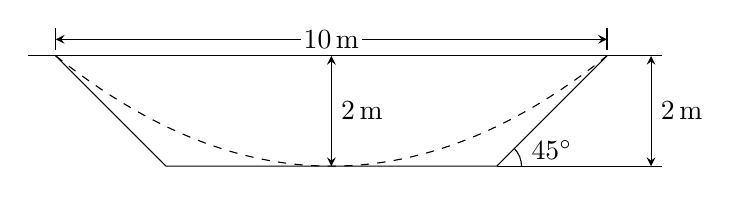
\begin{tikzpicture}[scale=0.7,>=stealth]
  \draw (-5,2)--(-3,0)--(3,0)--(5,2);
  \draw (-5.5,2)--(5.5,2);
  \draw[dashed,domain=-5:5,samples=100] plot (\x,{0.08*\x*\x});
  \draw[<->] (-5,2.3)--(5,2.3) node[midway,fill=white,inner sep=1pt] {$10\,\mathrm{m}$};
  \draw (-5,2.1)--(-5,2.5) (5,2.1)--(5,2.5);
  \draw[<->] (0,0)--(0,2) node[midway,right] {$2\,\mathrm{m}$};
  \draw[<->] (5.8,0)--(5.8,2) node[midway,right] {$2\,\mathrm{m}$};
  \draw (3,0)--(6,0) (5,2)--(6,2);
  \draw (3.45,0) arc (0:45:0.45);
  \node at (4.0,0.30) {$45^\circ$};
\end{tikzpicture}
\end{center}
\nopagebreak[4]
\end{question}
\gkpart{三、解答题}

\begin{question}
\gkti{17}

$\triangle ABC$ 的内角 $A,B,C$ 所对的边分别为 $a,b,c$。向量 $\boldsymbol m=(a,\sqrt3b)$ 与 $\boldsymbol n=(\cos A,\sin B)$ 平行。

（1） 求 $A$；

（2） 若 $a=\sqrt7$，$b=2$，求 $\triangle ABC$ 的面积。

\Needspace{0.4\textheight}
\end{question}
\begin{question}
\gkti{18}

如图 1，在直角梯形 $ABCD$ 中，$AD\parallel BC$，$\angle BAD=\frac\pi2$，$AB=BC=1$，$AD=2$，$E$ 是 $AD$ 的中点，$O$ 是 $AC$ 与 $BE$ 的交点。将 $\triangle ABE$ 沿 $BE$ 折起到 $\triangle A_1BE$ 的位置，如图 2。

（1） 证明：$CD\perp$ 平面 $A_1OC$；

（2） 若平面 $A_1BE\perp$ 平面 $BCDE$，求平面 $A_1BC$ 与平面 $A_1CD$ 夹角的余弦值。
\nopagebreak[4]
\begin{center}% 2015 年陕西卷（理科）第 18 题：折叠前的直角梯形与折叠后的四棱锥（依固定扫描页重绘，只画拓扑与标号，不按比例）
\begin{tikzpicture}[scale=0.85]
  % 图 1：直角梯形 ABCD，E 为 AD 中点，O 为 AC 与 BE 的交点
  \coordinate (A) at (0,2);
  \coordinate (B) at (0,0);
  \coordinate (C) at (2,0);
  \coordinate (D) at (4,2);
  \coordinate (E) at (2,2);
  \coordinate (O) at (1,1);
  \draw (A)--(D)--(C)--(B)--cycle;
  \draw (A)--(C);
  \draw (B)--(E);
  \node[above left] at (A) {$A$};
  \node[below left] at (B) {$B$};
  \node[below] at (C) {$C$};
  \node[above right] at (D) {$D$};
  \node[above] at (E) {$E$};
  \node[left] at (O) {$O$};
  \node at (2,-1.05) {图 1};
  % 图 2：折叠后所得四棱锥 A1-BCDE
  \begin{scope}[xshift=5.4cm]
    \coordinate (A1) at (0.9,3.0);
    \coordinate (B2) at (0.2,0.2);
    \coordinate (C2) at (2.2,0.2);
    \coordinate (D2) at (3.4,1.4);
    \coordinate (E2) at (1.4,1.4);
    \coordinate (O2) at (0.8,0.8);
    % 可见侧棱与底边：实线
    \draw (A1)--(B2);
    \draw (A1)--(C2);
    \draw (A1)--(D2);
    \draw (B2)--(C2);
    \draw (C2)--(D2);
    % 被遮挡的棱与辅助线：虚线
    \draw[dashed] (A1)--(E2);
    \draw[dashed] (D2)--(E2);
    \draw[dashed] (A1)--(O2);
    \draw[dashed] (B2)--(O2);
    \draw[dashed] (O2)--(E2);
    \draw[dashed] (O2)--(C2);
    \node[above] at (A1) {$A_{1}(A)$};
    \node[below left] at (B2) {$B$};
    \node[below] at (C2) {$C$};
    \node[right] at (D2) {$D$};
    \node[above left] at (E2) {$E$};
    \node[below] at (O2) {$O$};
    \node at (1.7,-0.75) {图 2};
  \end{scope}
\end{tikzpicture}
\end{center}
\nopagebreak[4]
\end{question}
\begin{question}
\gkti{19}

设某校新、老校区之间开车单程所需时间为 $T$，$T$ 只与道路畅通状况有关，对其容量为 100 的样本进行统计，结果如下：

\begin{center}
\begin{tabular}{lrrrr}
\toprule
$T$（分钟） & 25 & 30 & 35 & 40 \\
\midrule
频数（次） & 20 & 30 & 40 & 10 \\
\bottomrule
\end{tabular}
\end{center}

（1） 求 $T$ 的分布列与数学期望 $ET$；

（2） 刘教授驾车从老校区出发，前往新校区做一个 50 分钟的讲座，结束后立即返回老校区，求刘教授从离开老校区到返回老校区共用时间不超过 120 分钟的概率。

\Needspace{0.4\textheight}
\end{question}
\begin{question}
\gkti{20}

已知椭圆 $E:\frac{x^2}{a^2}+\frac{y^2}{b^2}=1$（$a>b>0$）的半焦距为 $c$，原点 $O$ 到经过两点 $(c,0)$，$(0,b)$ 的直线的距离为 $\frac12c$。

（1） 求椭圆 $E$ 的离心率；

（2） 如图，$AB$ 是圆 $M:(x+2)^2+(y-1)^2=\frac52$ 的一条直径，若椭圆 $E$ 经过 $A,B$ 两点，求椭圆 $E$ 的方程。
\nopagebreak[4]
\begin{center}% 固定源第20题：椭圆与圆及其直径，示意图
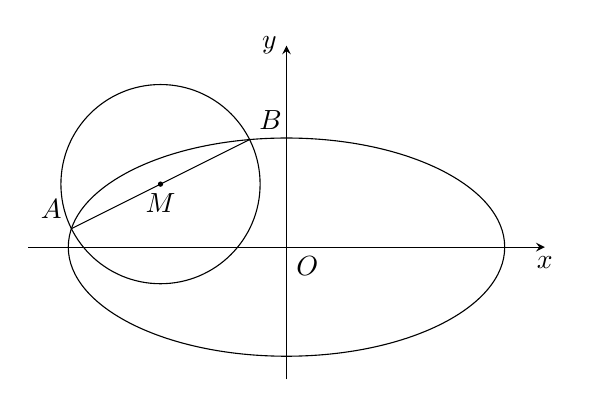
\begin{tikzpicture}[scale=0.8,>=stealth]
  \draw[->] (-4.1,0)--(4.1,0) node[below] {$x$};
  \draw[->] (0,-2.1)--(0,3.2) node[left] {$y$};
  \draw (0,0) ellipse ({sqrt(12)} and {sqrt(3)});
  \draw (-2,1) circle ({sqrt(2.5)});
  \coordinate (A) at ({-2-sqrt(2)},{1-sqrt(0.5)});
  \coordinate (B) at ({-2+sqrt(2)},{1+sqrt(0.5)});
  \draw (A)--(B);
  \fill (-2,1) circle (1.2pt);
  \node[above left] at (A) {$A$};
  \node[above right] at (B) {$B$};
  \node[below] at (-2,1) {$M$};
  \node[below right] at (0,0) {$O$};
\end{tikzpicture}
\end{center}
\nopagebreak[4]
\end{question}
\begin{question}
\gkti{21}

设 $f_n(x)$ 是等比数列 $1,x,x^2,\cdots,x^n$ 的各项和，其中 $x>0$，$n\in\mathbb N$，$n\geq2$。

（1） 证明：函数 $F_n(x)=f_n(x)-2$ 在 $(\frac12,1)$ 内有且仅有一个零点（记为 $x_n$），且 $x_n=\frac12+\frac12x_n^{n+1}$；

（2） 设有一个与上述等比数列的首项、末项、项数分别相同的等差数列，其各项和为 $g_n(x)$，比较 $f_n(x)$ 和 $g_n(x)$ 的大小，并加以证明。

\Needspace{0.4\textheight}
\end{question}
\begin{question}
\gkti{22}

如图，$AB$ 切 $\odot O$ 于点 $B$，直线 $AO$ 交 $\odot O$ 于 $D,E$ 两点，$BC\perp DE$，垂足为 $C$。

（1） 证明：$\angle CBD=\angle DBA$；

（2） 若 $AD=3DC$，$BC=\sqrt2$，求 $\odot O$ 的直径。
\nopagebreak[4]
\begin{center}% 2015 年陕西卷（理科）第 22 题：圆的切线与割线（依固定扫描页重绘，只画拓扑与标号，不按比例）
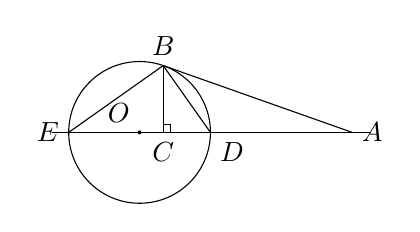
\begin{tikzpicture}[>=stealth,scale=0.6]
  % 圆 O
  \draw (0,0) circle (1.5);
  \fill (0,0) circle (1.2pt);
  \node[above left] at (0,0) {$O$};
  % 割线 A-D-C-O-E
  \draw (-1.85,0)--(4.9,0);
  \coordinate (E) at (-1.5,0);
  \coordinate (C) at (0.5,0);
  \coordinate (D) at (1.5,0);
  \coordinate (A) at (4.5,0);
  \coordinate (B) at (0.5,1.414);
  % 切线与弦
  \draw (B)--(A);
  \draw (B)--(E);
  \draw (B)--(D);
  \draw (B)--(C);
  % 直角标记
  \draw (0.5,0.16)--(0.66,0.16)--(0.66,0);
  % 标号
  \node[above] at (B) {$B$};
  \node[left] at (E) {$E$};
  \node[below] at (C) {$C$};
  \node[below right] at (D) {$D$};
  \node[right] at (A) {$A$};
\end{tikzpicture}
\end{center}
\nopagebreak[4]
\end{question}
\begin{question}
\gkti{23}

在直角坐标系 $xOy$ 中，直线 $l$ 的参数方程为 $\begin{cases}x=3+\frac12t,\\y=\frac{\sqrt3}{2}t,\end{cases}$（$t$ 为参数），以原点为极点，$x$ 轴正半轴为极轴建立极坐标系，$\odot C$ 的极坐标方程为 $\rho=2\sqrt3\sin\theta$。

（1） 写出 $\odot C$ 的直角坐标方程；

（2） $P$ 为直线 $l$ 上一动点，当 $P$ 到圆心 $C$ 的距离最小时，求 $P$ 的直角坐标。

\end{question}
\begin{question}
\gkti{24}

已知关于 $x$ 的不等式 $|x+a|<b$ 的解集为 $\{x\mid2<x<4\}$。

（1） 求实数 $a,b$ 的值；

（2） 求 $\sqrt{at+12}+\sqrt{bt}$ 的最大值。

\end{question}